\newpage
\section{Durchführung und Versuchsaufbau}



 \subsection{Versuchsaufbau}

    \subsubsection{Optischer Aufbau}

    \noindent Um zu gewährleisten, dass monochromatisches Licht genutzt wird, wird der in Abbildung \ref{img:linse} dargestellte Aufbau verwendet.


    \begin{figure}[H]
        \centering
        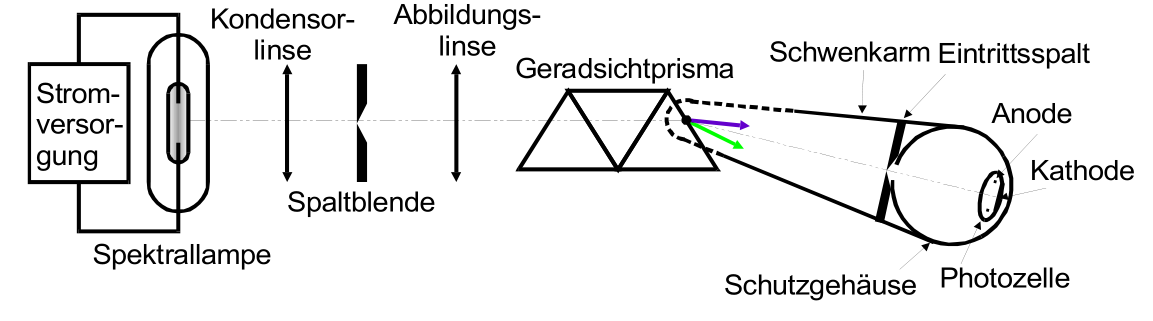
\includegraphics[width=0.7\textwidth]{latex/images/Optiken.PNG}
        \caption{Der optische Aufbau, welcher das Licht einer Spektrallampe aufspaltet  \protect \cite{500}.}
        \label{img:linse}
    \end{figure}

    \noindent Die Spektrallampe erzeugt hierbei Licht, welches von der Kondensorlinse gebündelt und durch die Spaltblende läuft.
    Anschließend wird das Licht wieder von der Abbildungslinse auf den Geradsichtprisma gebündelt, welcher das Licht in seine einzelnen Wellenlängen aufspaltet.
    Der Schwenkarm kann nun genutzt werden um die gewünschte Frequenz des Lichts auf die Photozelle strahlen zu lassen.\\
    Der reale Aufbau ist in Abbildung \ref{img:aufbau} zu finden.
    Die wichtigsten Emissionslinien und Farben einer Quecksilberlampe sind in der folgenden Tabelle zu finden.

    \begin{figure}[H]
        \centering
        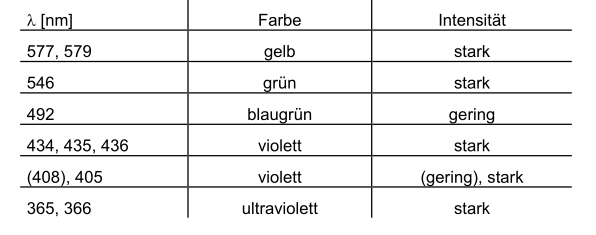
\includegraphics[width=0.6\textwidth]{latex/images/Hg.PNG}
        \caption{Die wichtigsten Linien einer Hg-Lampe\protect \cite{500}.}
        \label{img:Hg}
    \end{figure}

    \subsubsection{Elektrischer Aufbau }

    Um mit der Gegenfeldmethode den Fotoeffekt zu untersuchen wird sie an ein Digitalvoltmeter angeschlossen. 
    Damit können dann unterschiedliche Potentiale angelegt. 
    Zusätzlich wird an dei Fotozelle auch noch ein Picoamperemeter angeschlossen um die kleinen, von der Photozelle abfließenden Ströme messen zu können.\\
    Da die Ströme so klein sind sollte das Kabel von der Zelle zum Amperemeter ein Koaxialkabel oder eine ander geerdete Abschirmung sein, so dass die Messung nicht durch externe elektrische Felder beeinträchtigt werden kann.\\
    Zu sehen ist dieser Aufbau schematisch dargestellt in der folgenden Abbildung \ref{img:schem}.



    \begin{figure}[h]
        \centering
        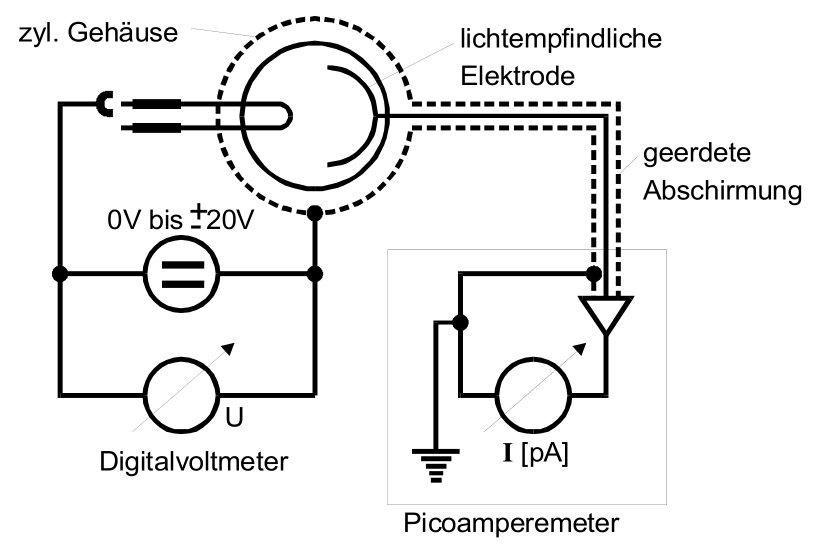
\includegraphics[width=0.6\textwidth]{latex/images/Schaltbild.PNG}
        \caption{Eine Photozelle in einem Schaltkreis zur Untersuchung des Photoeffekts\protect \cite{500}.}
        \label{img:schem}
    \end{figure}


\subsection{Durchführung}

Zuallererst wird auf die Photozelle das monochromatische Licht der Frequenz $578 \si{\nano\metre}$ gerichtet. 
Anschließend werden für diese Wellenlänge auf einem Spannungsintervall von $-20 \si{\volt}$ bis $20 \si{\volt}$ die Photoströme gemessen.\\\\
Zusätzlich werden für andere Spektrallinien die Abhängigkeit des Photostroms von der angelegten Gegenspannung gemessen.\\
Dabei soll bis zur Grenzspannung gemessen werden. 
Zusätzlich sollte beachtet werden, dass für niederenergetisches Licht, wie rot oder gelb, eventuell auch leichte beschleunigende Spannung angelegt werden müssen.
Dies dient dazu um so viele Messwerte zu generieren, dass sie der Auswertung genügen.
